\label{sec:intro}

Many real-world stochastic planning problems involving resources,
time, or spatial configurations naturally use continuous variables in
both their state and action representation.  For example, in a
\MarsRover\ problem~\cite{bresina02}, a rover must navigate within a
continuous spatial environment and carry out assigned scientific
discovery tasks; in \InventoryControl\ problems~\cite{Mahootchi2009}
for continuous resources such as petroleum products, a business must
decide what quantity of each item to order subject to uncertain
demand, (joint) capacity constraints, and reordering costs; and in
\WaterReservoir\ problems~\cite{reservoir}, a utility must manage continuous
reservoir water levels in continuous time to avoid underflow 
while maximizing electricity generation revenue.

Previous work on \emph{exact} solutions to multivariate continuous
state \emph{and} action settings has been quite limited.  There are
well-known exact solutions in the control theory literature for the
case of linear-quadratic Gaussian (LQG) control~\cite{lqgc}, i.e.,
minimizing a quadratic cost function subject to linear dynamics with
Gaussian noise in a partially observed setting.  However, the
transition dynamics and reward (or cost) for such problems 
cannot be piecewise --- a crucial limitation preventing the application
of such solutions to many planning and operations research problems. 

In this paper, we provide an exact \emph{symbolic dynamic programming} (SDP)
solution to a useful subset of continuous state and action Markov
decision processes (CSA-MDPs) with \emph{multivariate} continuous
state and actions, discrete noise, \emph{piecewise} linear dynamics,
and \emph{piecewise} linear (or restricted \emph{piecewise} quadratic)
reward.  To be concrete about the form of CSA-MDPs we can solve with
our SDP approach, let us formalize a simple \MarsRover\
problem:\footnote{For purposes of concise exposition and explanation
of the optimal value function and policy, this CSA-MDP example uses
continuous univariate state and action and deterministic transitions;
the empirical results will later discuss a range of CSA-MDPs with
multivariate continuous state and action and stochastic transitions.}

\begin{example*}[\MarsRover]
\label{ex:marsrover}
A Mars Rover state consists of its continuous position $x$ along a
given route.  In a given time step, the rover may move a 
continuous distance $y \in [-10,10]$.  The rover receives its greatest
reward for taking a picture at $x=0$, which quadratically decreases
to zero at the boundaries of the range $x \in [-2,2]$.  The rover will
automatically take a picture when it starts a time step within the
range $x \in [-2,2]$ and it only receives this reward once.
\end{example*}
Using boolean variable $b \in \{0,1\}$ to indicate if the picture has
already been taken ($b=1$), $x'$ and $b'$ to denote 
post-action state, and $R$ to denote reward, we 
express the \MarsRover\ CSA-MDP using piecewise dynamics and reward:
\begin{align} 
\hspace{-2.8mm} P(b'\sq=\sq1|x,b) & = 
\begin{cases}
b \lor (x \geq -2 \land x \leq 2): & \sqm 1.0\\
\neg b \land (x < -2 \lor x > 2):  & \sqm 0.0
\end{cases} \label{eq:mr_discrete_trans} \\
\hspace{-2.8mm} P(x'|x,y) & = \delta \left( x' - \begin{cases}
y \geq -10 \land y \leq 10 : & \hspace{-2mm} x + y \\
y < -10 \lor y > 10 : & \hspace{-2mm} x
\end{cases}
\right) \label{eq:mr_cont_trans} \\
\hspace{-2.8mm} R(x,b) & = \begin{cases}
\neg b \land x \geq -2 \land x \leq 2 : & 4 - x^2 \\
b \lor x < -2 \lor x > 2 : & 0
\end{cases} \label{eq:mr_reward}
\end{align}
Then there are two natural questions that we want to ask:
\begin{enumerate}
\item[(a)] What is the optimal form of value that can be 
obtained from any state over a fixed time horizon?
\item[(b)] What is the corresponding closed-form optimal policy?
\end{enumerate}
% Be nice to include that this is a breakthrough for deterministic
% systems as well

%%%%%%%%%%%%%%%%%%%%%%%%%%%%%%%%%%%%%%%%%%%%%%%%%%%%%%%%%%%%%%%%%%%%%%%%%%
\begin{figure}[t!]
\centering
%\subfigure{
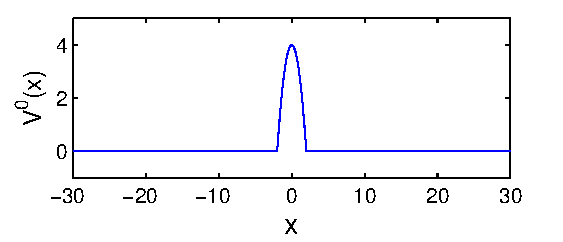
\includegraphics[width=0.35\textwidth]{Figures/v1_mr.pdf}\\
\vspace{-1mm}
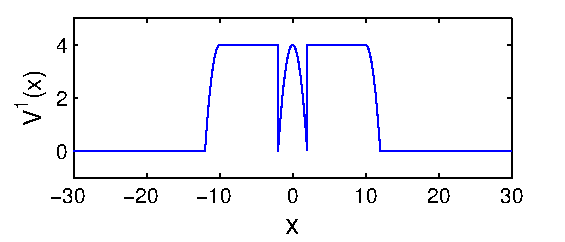
\includegraphics[width=0.35\textwidth]{Figures/v2_mr.pdf}\\
\vspace{-1mm}
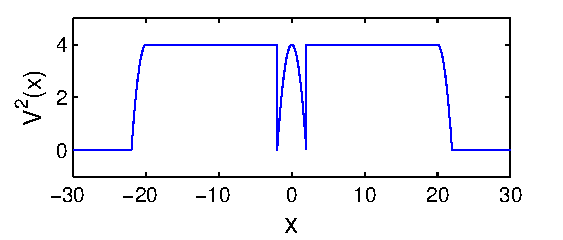
\includegraphics[width=0.35\textwidth]{Figures/v3_mr.pdf}
\vspace{-3mm}
\caption{\footnotesize Optimal sum of rewards (value) 
$V^t(x)$ for $b = 0 \, 
(\false)$ for time horizons (i.e., decision stages remaining) $t=0$,
$t=1$, and $t=2$ on the \MarsRover\ problem.  For $x \in [-2,2]$, the
rover automatically takes a picture and receives a reward quadratic in
$x$.  We initialized $V^0(x,b) = R(x,b)$; for $V^1(x)$, the rover achieves
non-zero value up to $x = \pm 12$ and for 
$V^2(x)$, up to $x = \pm 22$.}
\label{fig:opt_graph}
\vspace{-3mm}
\end{figure}
%%%%%%%%%%%%%%%%%%%%%%%%%%%%%%%%%%%%%%%%%%%%%%%%%%%%%%%%%%%%%%%%%%%%%%%%%%

To get a sense of the form of the optimal solution to problems such as
\MarsRover, we present the 0-, 1-, and 2-step time horizon solutions
for this problem in Figure~\ref{fig:opt_graph}; further, in symbolic
form, we display both the 1-step time horizon value function (the
2-step is too large to display) \emph{and} corresponding optimal
policy in Figure~\ref{fig:opt_val_pol}.  Here, the piecewise nature of
the transition and reward function leads to piecewise
structure in the value function and policy.  Yet despite the intuitive and
simple nature of this result, we are unaware of prior methods that can
produce such exact solutions.

To this end, we extend the previous SDP framework
of~\cite{sanner_uai11} to the case of continuous actions to obtain the
\emph{optimal closed-form} value function and policy for the
class of CSA-MDPs described previously (as well as the useful
deterministic subset).
As the fundamental technical contribution of the paper, we
show how the continuous action maximization step in the dynamic programming
backup can be evaluated optimally and symbolically --- a task which
amounts to \emph{symbolic} constrained optimization subject to
unknown state parameters; we further integrate this technique to work
with an efficient and compact data structure for SDP --- the extended
algebraic decision diagram (XADD).  
In addition to the solution of the nonlinear \MarsRover\
planning example above, we demonstrate empirical results on
\WaterReservoir\ and \InventoryControl\ domains from operations research
to show the \emph{first automated exact solution} to these problems.
%We additionally remark that all of the results in this paper apply to
%the deterministic subset of CSA-MDPs hence also providing exact
%solutions for continuous state and action deterministic planning.

%%%%%%%%%%%%%%%%%%%%%%%%%%%%%%%%%%%%%%%%%%%%%%%%%%%%%%%%%%%%%%%%%%%%%%%%%%
\begin{figure}[t!]
\centering
%\subfigure{
\hspace{-1mm}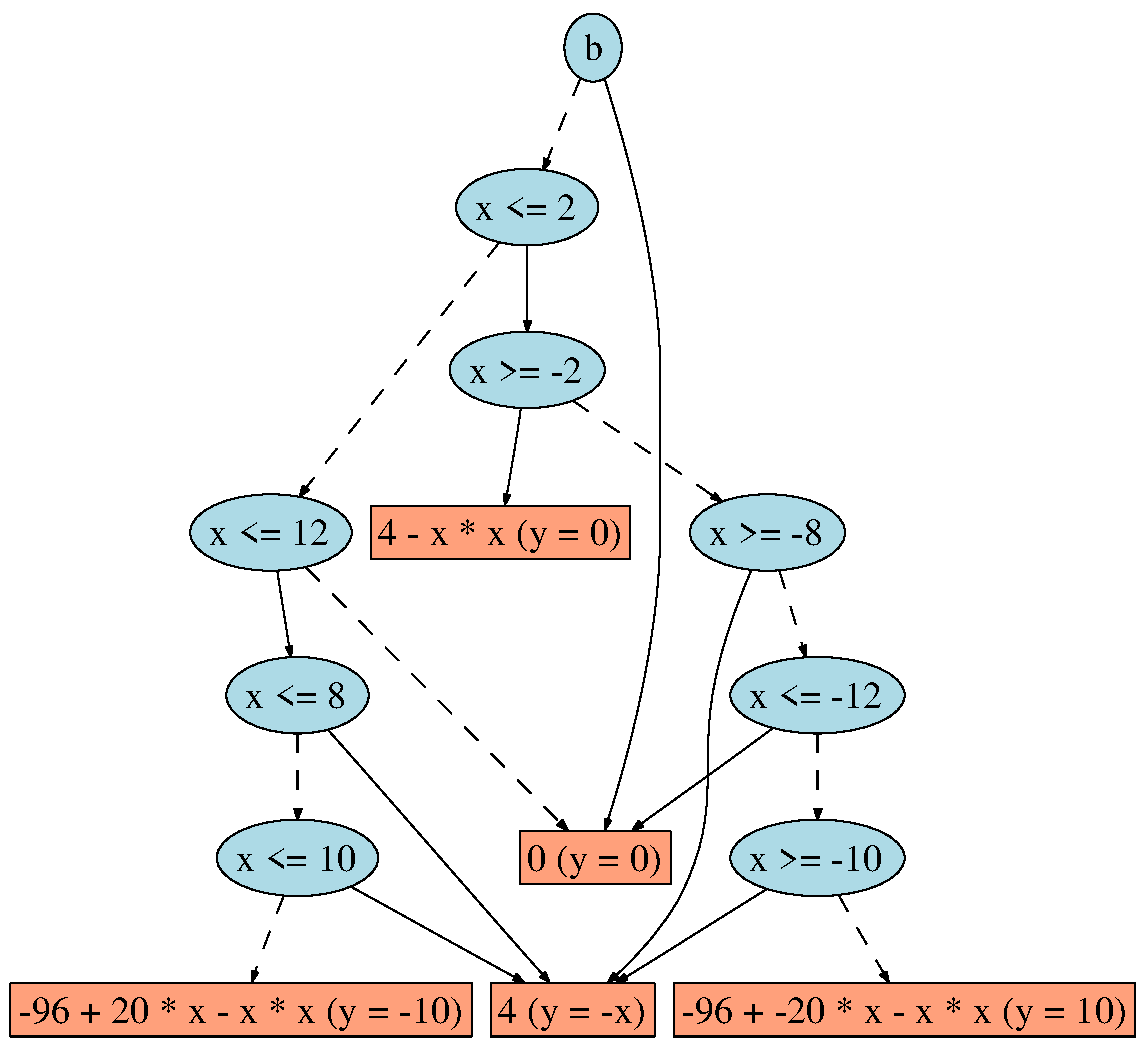
\includegraphics[width=0.43\textwidth]{Figures/v2_mr_dd.pdf}
\vspace{-1mm}
\caption{\footnotesize Optimal value function $V^1(x)$ for the
\MarsRover\ problem represented as an extended algebraic decision
diagram (XADD).  Here the solid lines represent the $\true$ branch for
the decision and the dashed lines the $\false$ branch.  To evaluate
$V^1(x)$ for any state $x$, one simply traverses the diagram in a
decision-tree like fashion until a leaf is reached where the
non-parenthetical expression provides the \emph{optimal value} and the
parenthetical expression provides the \emph{optimal policy} 
($y = \pi^{*,1}(x)$) to achieve value $V^1(x)$.}
\label{fig:opt_val_pol}
\vspace{-3mm}
\end{figure}
%%%%%%%%%%%%%%%%%%%%%%%%%%%%%%%%%%%%%%%%%%%%%%%%%%%%%%%%%%%%%%%%%%%%%%%%%%
